\subsubsection{System response}
The implementation of the control module was made using the modified speed algorithm mentioned and explained in \ref{sec:des-pid}.\\
The tests for this module consists in the comparison between the results obtained and simulated in \ref{sec:des-sim-res}.\\
Starting with speed reference = 1 m/s and $\theta=0~\si{rad}$:
\begin{figure}[!h]
\centering
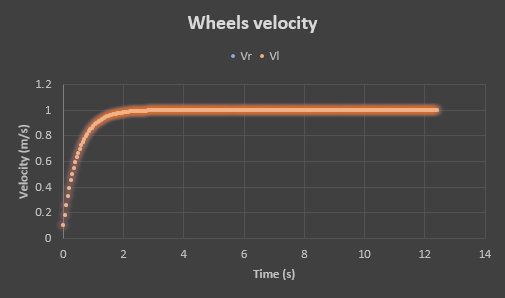
\includegraphics[width=0.7\textwidth]{./img/testv1t0.PNG}
\caption {\label{fig:test - vel0}Wheels velocity v=1m/s,$\theta = 0~\si{rad}$}
\end{figure}
In the figure \ref{fig:test - vel0} shows that the velocity of both wheels reaches the reference value in nearly 1.5 seconds, while in the simulation \ref{fig:sim1 - vel} it takes about 3 seconds. This discrepancy is due to the controller in use. The simulations  were made using the PID block provided by Simulink, while in the implementation, the controller algorithm used was as mentioned before, the modified speed algorithm. With this algorithm the behavior of the car is the same as with the traditional PID, but faster.
\begin{figure}[!h]
\centering
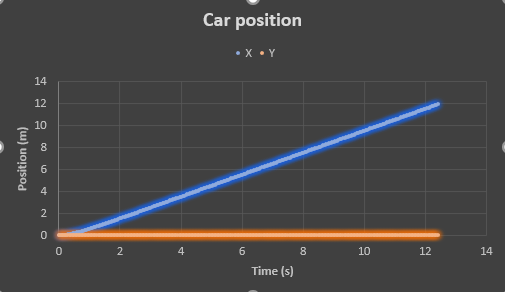
\includegraphics[width=0.7\textwidth]{./img/testx1t0.PNG}
\caption {\label{fig:test - xy0}Position v=1m/s,$\theta = 0~\si{rad}$}
\end{figure}
In the figure \ref{fig:test - xy0} it can be observed that the position of the car is the same as in the simulation \ref{fig:sim1 - pos}.
\newline
With speed reference = 1m/s and $\theta = 0.1~\si{rad}$:
\begin{figure}[!h]
\centering
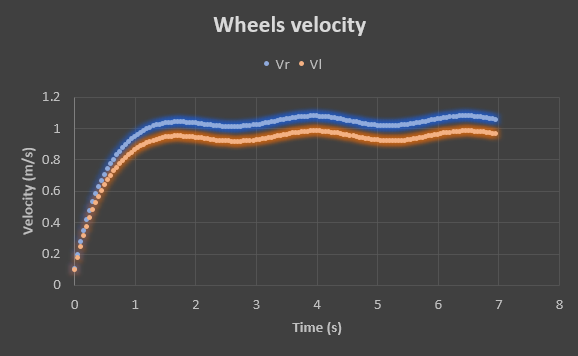
\includegraphics[width=0.7\textwidth]{./img/testv1t01.PNG}
\caption {\label{fig:test - vel01}Wheels velocity v=1m/s,$\theta = 0.1~\si{rad}$}
\end{figure}
In the figure \ref{fig:test - vel01} comparing to \ref{fig:sim2 - vel} it's possible to see that once again the time it takes to reach steady state is smaller for the reason mention before. In the implemented algorithm it's also possible to see that the steady value of the velocity of both wheels has a ripple around the reference value. 
\begin{figure}[!h]
\centering
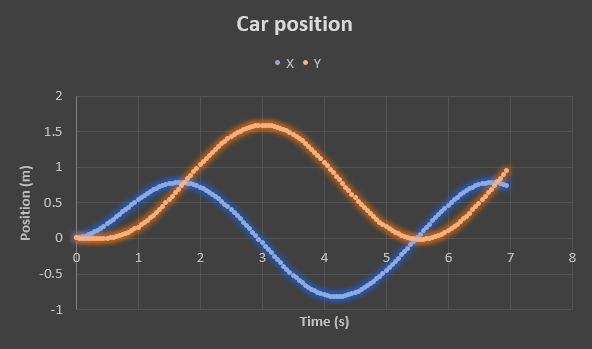
\includegraphics[width=0.7\textwidth]{./img/testx1t01.PNG}
\caption {\label{fig:test - xy01}Position v=1m/s,$\theta = 0.1~\si{rad}$}
\end{figure}
In the figure \ref{fig:test - xy01} it is present the position of the car. In comparison to the simulated \ref{fig:sim2 - pos} it is possible to see that the results are the same, thus validating the implementation.
\subsubsection{Obstacle Avoidance Through Odometric Sensors}
The car composed by 9 odometric sensors radially distributed, 40 degrees apart.\\
In order to test if the car can avoid obstacles, the values for the sensors were generated, and the behavior of the car was as follows:
\begin{figure}[!h]
\centering
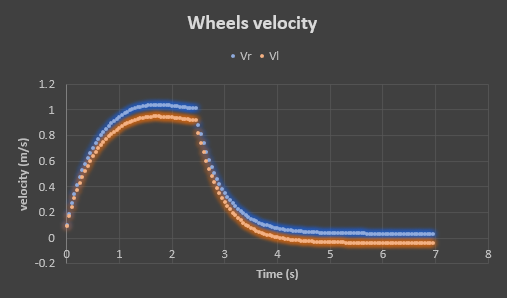
\includegraphics[width=0.7\textwidth]{./img/testodovel.PNG}
\caption {\label{fig:test - odovel}Wheels velocity}
\end{figure}

\begin{figure}[!h]
\centering
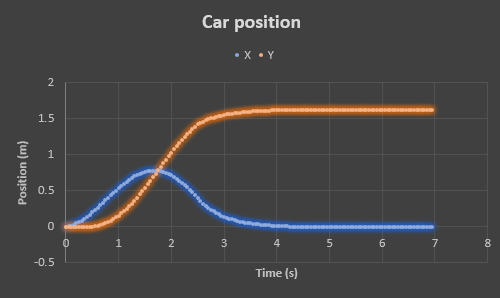
\includegraphics[width=0.7\textwidth]{./img/testodoxy.PNG}
\caption {\label{fig:test - odoxy}Car position}
\end{figure}

In the figure \ref{fig:test - odovel} it is possible to see that at t=2.5 seconds the velocity of both wheels starts decreasing until they reach a value near 0 m/s. Even though the velocity of both wheels is not exactly 0 m/s, the values are too small to break the inertia of the wheels, so the car effectively stops.
In the figure \ref{fig:test - odoxy} it is possible to see that the position of the car remains the same after the decrease of the velocity of the wheels, proving that the car is not moving.